\documentclass[UTF8]{ctexart}
\usepackage[left=2.50cm, right=2.50cm, top=2.50cm, bottom=2.50cm]{geometry}
\usepackage{amsmath, amsfonts, amssymb}
\usepackage[english]{babel}
\usepackage{graphicx}
\usepackage{url}
\usepackage{bm}
\usepackage{indentfirst}
\usepackage{threeparttable}
\usepackage{multirow}
\usepackage{cite}
% \usepackage{booktabs}
\usepackage{listings}
\usepackage{algorithm}
\usepackage{float}
\usepackage{algorithmic}
\usepackage{inconsolata}
\usepackage{color}
\usepackage[explicit]{titlesec}
\usepackage{xcolor}
% \usepackage{abstract}
\usepackage{multicol}
\setlength{\parindent}{2em}
\CTEXsetup[format={\Large\bfseries}]{section}

\title{\textbf{一种基于区块链的的新型智能运输系统}}
\author{\sffamily 郑力文,余稼俊,何浩岚\\ \sffamily(电子科技大学,四川 \ 成都)}
% \author{\sffamily 李四}
\date{}

\newcommand\picturehere[2][1]{\centerline{\includegraphics[scale = #1]{#2}}}
\newcommand\picfig[1]{\centerline{\small \heiti #1 \songti }}


\begin{document}
  \maketitle
  \textbf{\kaishu摘 \ 要:\heiti  \small 如今外卖业务和物流业务都伴随着电子信息技术的发展而不断提升,两者实质上都是一种资源传递的行为,而本文设计并提出了一个采用EOS底层区块链技术的一种同时支持长途、短途的“人人可送”的智能货物运输平台。这个平台的目的是提高物流等平台的可靠性、数据安全性,同时结合推荐算法为用户、司机提供一种匹配模型,减少订单之间的等待时间,一定程度上避免“空车返回”的现象发生,进而提升资源的传递效率。最后我们提出采用星际文件系统以期避免分布式系统的造成的在节点设备上的存储限制问题。}
  \\
  \indent \textbf{\kaishu关键词:\heiti  \small 物流,区块链,智能合约,星际文件系统,效率}
  \pagestyle{plain}	% 去除页眉
  \\
  \\




  \titlespacing*{\section}{0pt}{1.2ex plus .0ex minus .0ex}{.9ex plus .2ex}
  \titlespacing*{\subsection}{0pt}{1.2ex plus .0ex minus .0ex}{.9ex plus .2ex}


\begin{multicols}{2}
  \setcounter{section}{-1}
  \section{引言}
    随着互联网时代的到来,不论是城市内短途的“跑腿”“外卖”服务还是跨市、跨省的长途运输服务都在迅速发展,而我国在这方面的需求量更是巨大。但同时,在一些高峰期“人找好车难”“车找货难”“空车返回”的现象也数见不鲜,这些都会产生资源闲置和运输费用成倍增加的问题。\\
    \indent 为了解决用户与送货者之间的信任问题,从而缓解“人找好车难”的问题,我们决定采用区块链技术。在2016年12月在国务院发布的《国务院关于印发“十三五”国家信息化规划通知》中第一次将区块链作为颠覆性技术、战略性前沿技术列入国家通知中\cite{ref1}。而区块链技术由于其特有的不易篡改、数据透明的特点,无疑可以很好地作用在物流方向上。以此缓解用户对于运货途中对于货物安全、运输时效的担忧。在这个分布式系统中,每个用户和运输者的终端设备就相当于一个参与节点,在其中共享数据。但是我们难以让每一个用户的设备都存储下链上的每一条数据,这样的成本是巨大的,因而我们打算采用星际文件系统(IPFS)来降低主链的数据存储成本。\\
    \indent 而为了提高资源利用率,减少“车找货难”“空车返回”等问题,我们决定设计一个推荐算法,用于匹配运货者(的车)与用户的传运需求。这里,我们希望采用一种基于车辆推荐的画像数据可用性判断方法\cite{ref2},不仅可以让用户与运货者之间做出快速且符合要求的相互选择,同时可以在上一次运输的目的地周围寻找以此为起点且以原出发地附近为终点的订单,从而减少“空车返回”现象的发生,减少在能源、时间上产生的无谓损失。\\
    \indent 本文将在第一章描述该平台的运作方式;第二、三章介绍其如何以EOS作为底层技术、IPFS作为存储方式;第四章将描述基于车辆算法的推荐算法。
  \section{新型平台模式设计与介绍}
  \subsection{区块链技术}
  目前区块链技术的开源项目如雨后春笋般有十分多的类型,这里比较了5种目前较流行的区块链项目(Bitcoin、Ethereum、Hyperledger、EOS、Corda)进行对比。\\
  \renewcommand{\tablename}{\small\heiti表\songti}
  \begin{table*}[htbp]
    \centering
    \caption{\small\heiti目前主流区块链项目对比\songti}
    \begin{tabular}{|c|c|c|c|c|c|}
      \hline
      项目名称 & 共识算法   & 去中心化程度 & 代币功能  & 智能合约 &速度 \\ \hline
      Bitcoin & PoW       & 高         & 有 & 不支持 & 慢\\ \hline
      Ethereum & PoW/PoS & 高 & 有 &支持 &较慢\\ \hline
      HyperledgerFabric & RAFT/BFT & 中 & 无 &支持 & 快\\ \hline
      EOS & DPoS & 中 & 有 &支持 &快\\ \hline
      Corda & Raft/BFT & 低 & 无 &支持 &快\\ \hline
    \end{tabular}
  \end{table*}
  \indent 由于我们的算法需要建立在智能合约的基础上,并且为了方便交易,我们也需要用到代币功能,且其交易速度应该够快以满足平台的计算和交易需求。同时为了更好地保证平台数据安全性,我们也希望其具有较高的去中心化水平。综合以上需求,采用EOS项目可以很好的实现这个平台。
  \subsection{功能性需求}
  我们将每一次订单发布到实现的过程分为3个部分:订单发布与接受部分、运输与信息共享部分、交易与评分模块。下面将分别详细描述这三个部分。
  \subsubsection{订单发布}
  订单发布又可以细分为有送货需求的用户发布订单和传输者(司机)发布订单。\\
  \indent 有送货需求的用户发布订单需要上传货物信息,包括货物的重量、体积、材质种类、货物价格、起点终点的地址等等。在上传信息之后,系统自动将这笔订单信息打包成一个区块,这个区块便是这个订单的创世区块,同时在用户进行数字签名后对其他节点进行广播,其他节点验证该区块信息正确性后将在自身节点上同步该订单信息。\\
  \indent 而传输者同时也可以发布或更改自己的车辆信息,从而在系统推荐算法中找到更适合自己的订单(或者让别人更快的找到自己)。由于链上的信息已经不可修改,所以每一次的信息发布或更改都会产生一个新的区块,而这也将在数字签名后想其他节点进行广播。
  \renewcommand{\figurename}{\heiti\small图\songti}
  \begin{figure}[H]
    \centering
    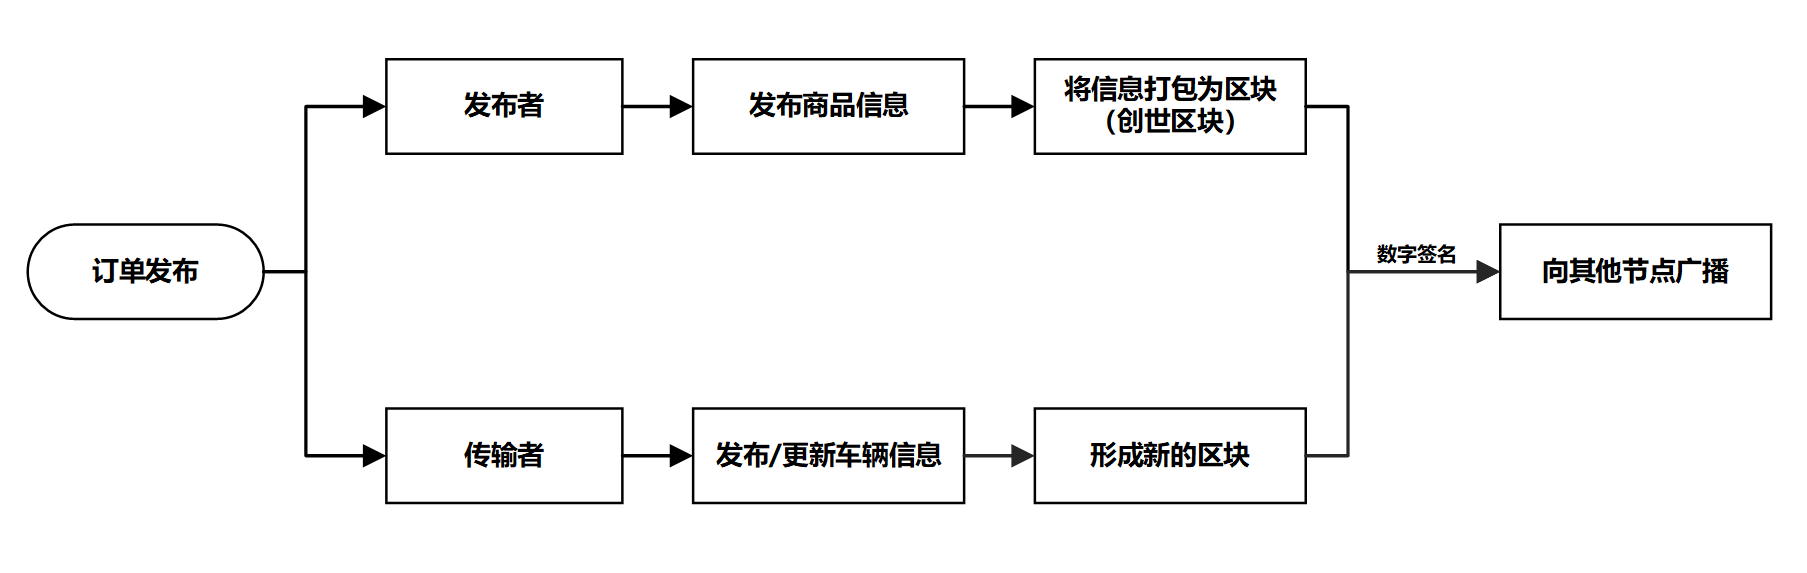
\includegraphics[width=1.1\linewidth]{image/order.png}
    % 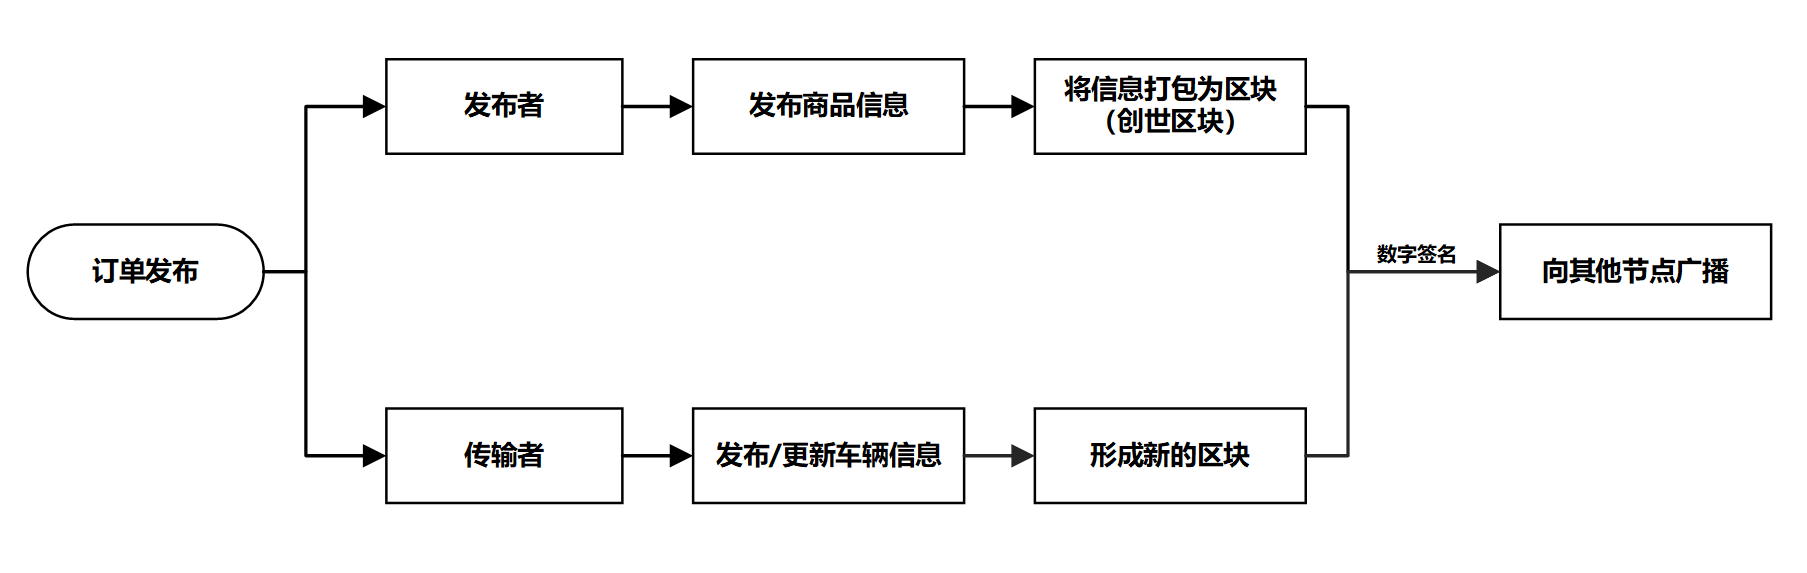
\includegraphics[scale=0.2]{image/order.png}
    \caption{\heiti\small订单发布示意图\songti}
  \end{figure}
  在订单发布后,系统后台自动运行车货匹配推荐算法。发布者可以看到根据推荐算法计算出的匹配程度由高到低的可用车主信息\footnote{这里的可用也可能指在马上执行完上一次任务的司机,且上一次任务的终点处于本次任务的起点。}。司机可向订单发布者发送接单申请,订单发布者也可以向司机发送接单申请。当另一方同意了接单申请后即进行双方即进行数字签名,将该成交订单向其他节点广播。
  \subsubsection{运输部分}
  运输部分建立在订单发布后司机已经接单的前提下,这部分可以对订单部分进行实时更新,包括检查订单状态、检查实时位置等操作。该部分流程如下。\\
  \indent 1、司机到订单指定起点位置,将要运输的货物装载。装载完成后,司机对该区块链上的运输信息进行数字签名,广播到其它节点。一旦检测到该过程结束,系统便会会这个订单生成一个用户的查询接口。\\
  \indent 2、在运输过程中,定位模块将对货物的位置信息(实质上是司机的终端设备的位置信息)进行实时更新,每一次的位置操作也都将更新到区块中,形成不可更改的货物位置追踪记录。\\
  \indent 3、当司机将货物送至指定地点时,让收货人进行验收,若验收成功,则对该订单信息进行数字签名,发布并等待其他节点验证。当上述操作完成之后,该订单确认送达,进入转账操作。
  \begin{figure}[H]
    \centering
    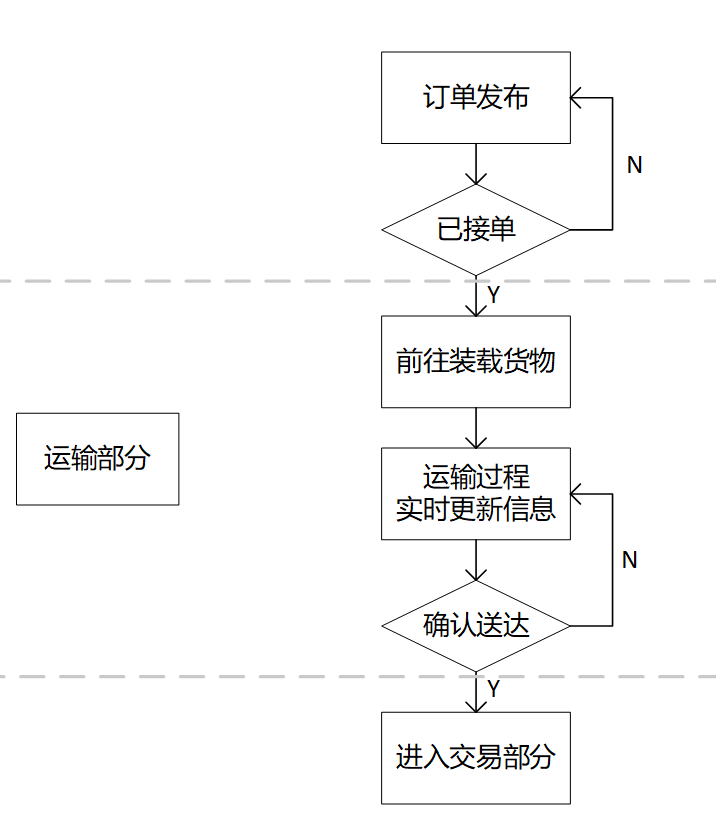
\includegraphics[scale=0.6]{image/transfer.png}
    \caption{\heiti\small运输部分流程示意图\songti}
  \end{figure}
  \subsubsection{交易部分}
  当用户确认物品已经安全送达后,系统会向发布用户提交转账申请。\\
  \indent 首先系统会判定发布者的对应的地址余额是否充足,当用户同意进行转账操作并且余额充足后,转账操作进行,订单发布者与司机账户对应余额减少或增加相应数量。转账操作结束后两个账户对此次操作进行数字签名并广播到其它节点。
  \subsection{推荐算法部分}
  该部分目的在于快速匹配与需要运送货物相符的车辆或为车辆匹配与之对应的货物订单。因此我们决定采用一种在优先满足硬性条件前提下的的基于车辆推荐的画像数据可用性判断方法结合匹配中的三种“软性条件匹配”模型\cite{ref3}——“线路选择模型”“合作关系模型”“隐性资源趋势模型”。这些推荐算法与模型将在后文中详细说明。
  \section{区块链技术在该平台中的应用}
  如上文所说,基于EOS项目免费试用、轻松调试、低延迟、串并行性能高的特点,我们在该平台中决定使用EOS进行智能合约的部署。该部分详细介绍了该项目在如何区块链上的部署与执行。
  \subsection{EOS介绍}
  \indent EOS和ETH的愿景大致相似,都是一个操作系统的底层。其中我们可以构建各种各样的智能合约应用。而EOS通过并行链和DPoS的方式解决了延迟大,和数据吞吐量小的难题。EOS的数据吞吐量理论可以达到百万TPS的数量级。该区块链不需要通过费用来加入与执行合约,大大降低了部署与运行的成本。\\
  \subsection{EOS账户}
  EOS自带基于角色权限管理和账户恢复功能的账户体系,是一种更加灵活的组织和管理账户的方式。EOS.IO软件允许帐户可被长度多达12个字符的唯一可读名称所引用。该名称由帐户的创建者选择。帐户创建者必须保留存储新帐户所需的RAM,直至新帐户存储令牌以保留其自己的RAM\cite{ref4}。EOS没有采用地址的形式而是采用账户的形式,这是EOS相对于以太坊和比特币的不同之处。每一个账户都为长度为12位\footnote[1]{事实上可以存在小于12位的账号,但长度小于12位的账号属于高级账号,系统每天进行只会进行最多一次高级账号的拍卖。如第一个拍卖的账户名"eos"价格高达50000EOS,现在价格已超过百万人民币},包含了英文字符'a'$\sim$'z'以及数字1$\sim$5,这样的优点在于将原来没有固定格式的长地址形式转换为人们容易记住的形式。\\
  \indent 重新回到考虑如何在我们设计的平台中使用EOS的优势来进行部署的问题。EOS账户中自带两个权限:owner与active\footnote[2]{还存在一个账户被盗后用于恢复账户的Recovery权限与用户自定义的权限,我们在这里不做考虑}。两者实质上都是私钥的形式。Owner权限代表了用户对账户的所有权,可以对账户进行任何修改。而active权限一般用于转移资金、执行智能合约、为DPoS机制中的区块生产者投票等等操作。事实上在EOS系统中智能合约也有类似的权限,我们在实现该运输平台的合约时便可运用这一特点。具体的说,我们可以在合约权限中设置阈值,每当有新的订单发布或转账操作要进行,我们就让该系统中所有账号进行验证,只有当最后认可该信息的节点数量大于事先设定的阈值时,该信息才最终会被更新到作业链上。通过这样的方式,我们可以确保数据的安全性以及真实性。\\
  \subsection{数字签名}
  在上文提到了其他节点用于验证信息真实性、确定身份、确定责任的方法便是数字签名,几乎全部区块链项目都采用了数字签名这一方法,EOS也不例外。在我们的系统中并不需要我们自己来构建数字签名的加密算法,但其作为几乎作业链中每一个流程都需要用到的东西,我们决定在这里介绍一下EOS中数字签名的过程。\\
  \indent 在上一小节中提到了EOS账户,而这一节中我们则介绍与之相对应的“钱包”。在EOS系统中,钱包与账户并不一一对应,相反它们可以存在一对多的关系,即一个钱包中可以管理许多账户,而这里账户的表现形式形式便为私钥。其关系可参照下图3。\\
  \begin{figure}[H]
    \centering
    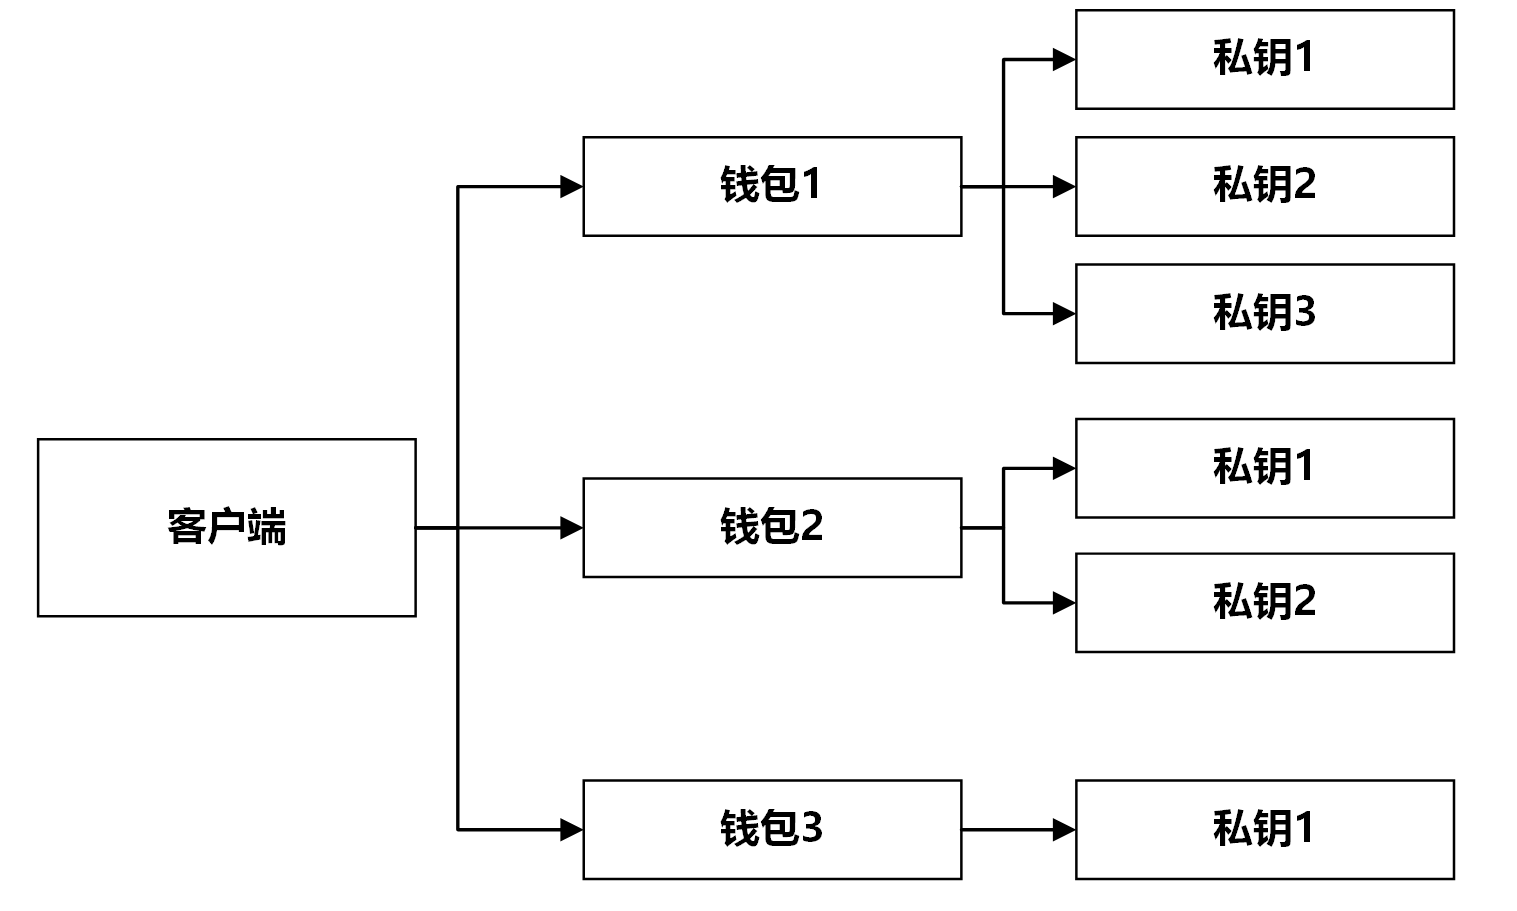
\includegraphics[width=\linewidth]{image/psw.png}
    \caption{\heiti\small钱包-私钥对应关系\songti}
  \end{figure}
  \indent 而数字签名的工作流程如图4所示。发送方对原始数据通过哈希计算数字摘要,接着使用非对称加密\footnote[1]{EOS中采用了椭圆曲线加密方式}中的私钥对其进行加密,然后将加密后的数据向其他节点广播。当接收方进行验证时,首先使用发送者公钥对数字签名进行解密,将原始信息的散列值与解密出的散列值对比,只有两者相同时签名验证才算通过。
  \begin{figure}[H]
    \centering
    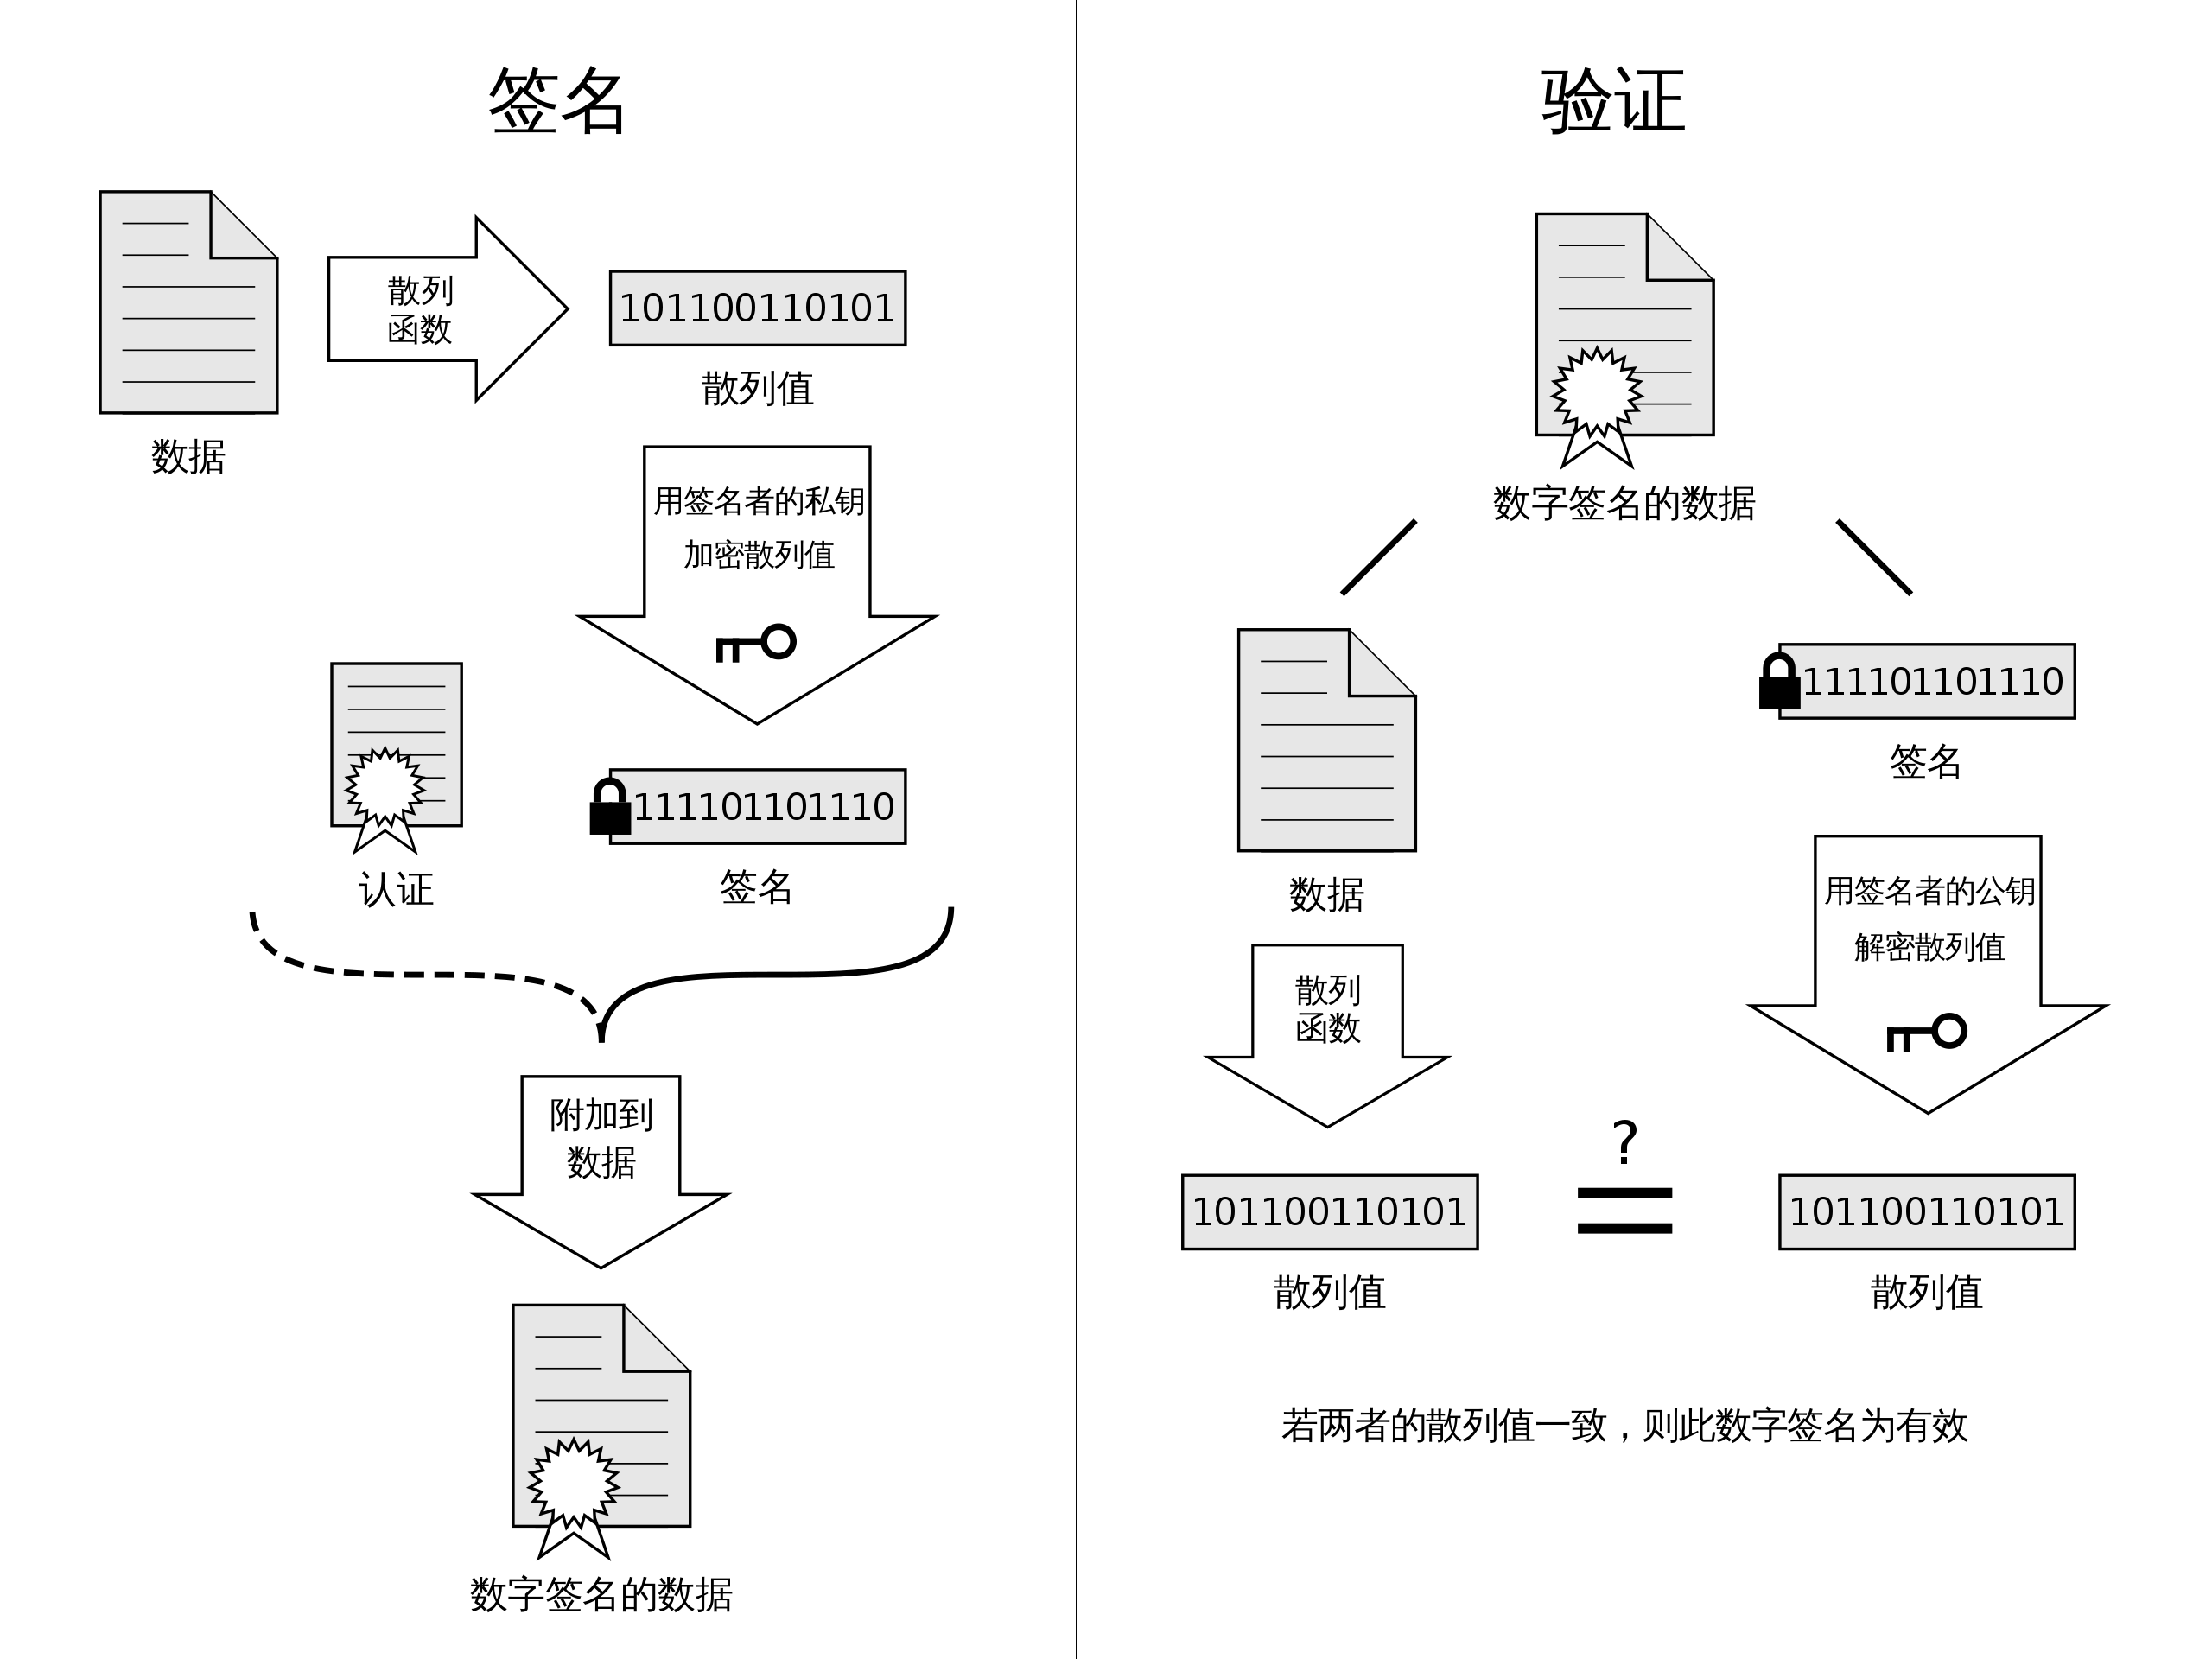
\includegraphics[width=\linewidth]{image/check.png}
    \caption{\heiti\small签名及签名验证的流程示意图\songti}
  \end{figure}

\section{IPFS在该平台中的应用}
\subsection{IPFS介绍}
IPFS(星际文件系统,Inter Planetary File System)是一个旨在创建持久且分布式存储和共享文件的网络传输协议。它是一种内容可寻址的对等超媒体分发协议。在IPFS网络中的节点将构成一个分布式文件系统。\\
\indent在本地IPFS 系统中的文件存在两种状态,分别为永久存储和缓存状态,使用PIN功能可以使永久存储状态和缓存状态互转换。IPFS 系统的寻址方式分为两种,一种是IPFS寻址(不可变内容寻址),由梅克尔有向无环图提供的基本内容寻址;还有一种是SIHPNS寻址(可变内容寻址),即节点将IPFS 数据发布到每个IPFS 节点的不可更改的IPFS 地址下,从而达到可变内容寻址的目的。
\subsection{应用与分析}
根据EOS白皮书的介绍,EOS将来会内置一个IPFS标准的文件系统\cite{ref5}\\
\indent 我们希望基于EOS开发货物传输平台,而基于EOS的交易量非常大, 0.5s会产生一个区块的数据。如果所有用户信息与交易数据全部记录在主链上,那么将会产生非常巨大的数据量,而通过IPFS可以极大地降低主链本身的数据存储成本。\\
\indent 此外,DApp在用户访问前端时需要静态的页面分发服务,它的前端文件目前是中心化的。通过把这些前端程序或者网站前端放到基于IPFS的文件存储上,只需要抵押一定的EOS代币,就可以实现Web服务的去中心化和低成本。\\
因此,我们可以将账户系统与交易系统放在EOS 主链上,将前端页面、车辆信息、司机信息、路线信息等信息、推荐算法和预处理信息等全部放在IPFS 上,确保低成本的同时进行了完整的体系架构。\\
\indent 而相比传统的数据中心化、难备份的储存方式,IPFS能够永久的、去中心化保存和共享文件,从而使我们的交易记录和用户信息全部得以永久安全储存,且便于我们查询溯源 ;在传统的数据存储中,数据是被直接储存的,安全性并不让人满意,而IPFS会对所有内容都进行加密与校验。我们通过EOS实现一个文件交易DApp,那么所有文件便可以通过IPFS存储,并用密钥加密来保证其安全性,用户也可以通过修改密钥可实现链上的产权转移达到文件交易的目的。此外,相比于传统的区块链,IPFS并不会要求每一个节点都存储所有的内容,节点的所有者可以自由选择想要维持的数据,在备份了自己的用户与交易数据之外,可以自愿的为其他的用户提供数据存储服务并从中活动利好,解决了传统区块链区块数据量巨大而每个节点都必须全部下载的痛点。
\section{模型建立与推荐算法}
该平台采用的推荐算法先根据目标重要性进行排序,选出其中较为重要的目标作为候选目标集,接着在候选目标集中按照目标的匹配度和相应规则不停地进行筛选,直至选出最优目标,即最终推荐集。我们将对目标的需求匹配分为两种:硬匹配与软匹配。硬匹配对应对目标较强的属性限制,如车辆类型、载重、车辆体积等;而软匹配对目标的属性制约并不强烈,但是对于决策有很好的辅助作用。由于算法难以直接对零散数据进行有效应用,我们从物流运输中抽象出了基础条件、线路选择、合作关系、隐性资源四个数学模型,并将数据结构化后再用算法进行推荐。
\subsection{模型构建}
\subsubsection{基础条件模型}
我们发现,运输车辆类型(卡车、面包车、电动车等)、车辆载重、车辆尺寸(长度、限高、体积)等基础条件对推荐范围有着直接的影响,属于硬性制约条件。此外,某些大型车对只能运输特定的货物,某些货物只能由特定的大型车运输。因此,将这些硬性条件抽象出一个基础条件模型,为进一步的硬匹配处理出结构化的数据。

该模型中的数据主要有车辆基本信息(车牌、类型、载重、尺寸、特定运输限制)、车辆司机基本信息(姓名、电话、驾龄、驾驶里程)、司机的运输偏好(长途/短途)等。

该模型处理数据的基本步骤如下:

第一步:进行数据清洗工作。如果出现同一辆车拥有多个id、车辆尺寸与类型不一致、联系人有多个等情况,则该车不可用,将此类无效数据清除。

第二步:对车辆基本信息进行去重处理。经过第一步清洗后,每辆车只对应一个车辆id,随即以注册时间距现在时间最近的车辆为基准,对每一个id的车辆基本信息进行去重处理。

第三步:对车辆类型进行校验处理。以该车在平台上最近的成交记录为基准,更新车辆的类型信息,对历史登记信息进行校验。新注册的车辆则需要上传机动车行驶证和机动车驾驶证信息,以便准确采集车辆类型信息。

第四步:对车辆司机的电话进行校验处理,以最近成交记录中的电话为基准,对所有车辆司机电话信息进行校验,以获得准确的联系人信息。

第五步:对平台上所有的车辆基本信息进行画像处理,并将全部车辆信息按结构体形式存储到车辆数据库中,方便推荐算法调用。

第六步:当收到推荐请求时,根据车辆需求信息进行筛选,去掉基础条件不符合的车辆,形成推荐车辆的候选集,并进行进一步筛选以形成最终的推荐范围。
\subsubsection{线路选择模型}
除了上述提到的基础硬性条件,现实中还存在许多软性条件限制。中长途运输不同于短途运输,常进行中长途运输的司机倾向于相对固定的货源和较为熟悉的路线,他们熟悉沿途高速收费情况、道路拥挤程度等,对目的地城市往往也比较熟悉。选择这些路线可以帮助司机准时安全地将货物送达。因此我们抽象出一个线路选择模型,帮助推荐算法根据不同的订单需求进行更加精准高效的推荐,提高推荐成功率。

该模型中的数据主要有车辆进行长途/短途运输的次数、车辆启发点、车辆终达点、订单沿途途径点位等。

该模型处理数据的基本步骤如下:

第一步:对车辆历史订单进行分析。由此初步确定车辆的偏好,如司机习惯于长途还是短途运输、经常途径哪些城市、常跑路线等。

第二步:对运输路线进行画像处理。以历史运单中的启发地和终达地为基础,统计出该车辆经常运输路线,并记录下对应的运输次数。

第三步:对途径城市进行画像处理。统计出历史订单中的启发地和终达地,并记录下城市被途径的次数。

第四步:建立城市之间的相似度地图。对每个城市和其周围一定范围内的城市建立相似关系,距离越近则相似度越高。之后进行线路匹配可以利用相似度排序进行更有效更准确的推荐。

第五步:对经基础条件模型筛选后得到的候选集中的车辆进行线路选择,根据订单需求的启发地和终达地进行匹配计算,若车辆的熟悉路线和这两个地点进行相似度匹配计算的值较高,则提高该车辆的推荐分值,最后根据分值进行综合排序,得到最适合的推荐集合。

\subsubsection{合作关系模型}
有些司机不一定具有相对固定的运输路线,而是拥有相对固定的货源地与合作厂商,并且和这些厂商或仓库有较高的熟悉与信任度。几乎每个厂商都有一批经常合作的运输司机,每个司机手中也常有经常联系的仓库与货源地。因此,我们抽象出一个合作关系模型,将订单推荐给与需求方有较强合作关系的司机,由此提高推荐的成功率。

该模型中的数据主要有司机id、货主id、合作次数、货源地地点等。

该模型处理数据的基本步骤如下:

第一步:基于历史订单,对所有货主(货源地)按司机id进行合作次数统计,并映射为合作关系强度。对于超过3个月的历史合作记录,降低其权重再进行统计。建立以货主为中心结点、司机为子结点的辐状图,边权重即为经加权计算后的有效合作次数。

第二步:根据订单需求的启发地和终达地,结合城市相似度地图,根据相似度和合作关系强度两个指标对各司机进行评分,城市相似度越高、合作关系越强,则评分越高。在合作关系足够强的情况下,允许存在启发地或终达地周边城市货源的合作司机评分高于本地货源的合作司机评分,由此可计算出更符合实际的结果。

第三步:对启发地和终达地及其周边货源地的合作司机按分值排序,对各序列中的司机进行综合总排序,选取分值高且与两地均有较强相关性的司机放入推荐集合。
\subsubsection{隐性资源模型}

我们发现,仅仅以车辆与启发地的距离进行推荐存在其片面性。因为车辆的行驶方向并不确定,对一个距离货源地很近但正在远离货源地的车辆进行推荐显然是不合理的。事实上,司机们常常在还未到终达地的时候就开始联系当地货源,因此对正在靠近货源地的车辆进行推荐有较高的成功率。同时,在货源地或其附近静止的车辆被推荐成功的机率也比较大。由此抽象出一个隐性资源模型。

该模型中的数据主要有车辆不同时刻的位置信息、车辆id。

该模型处理数据的基本步骤如下:

第一步:判断车辆位置。根据以生成的候选集中的车辆id去获取其位置,判断车辆是否在启发地周围,如果否则筛出候选集。

第二步:获取启发地周围未被占用车辆的id和位置,将其加入候选集。

第三步:对候选集中的车辆每隔10分钟记录一次位置信息,连续记录2小时。

第四步:根据记录下的2小时位置信息判断车辆是否为静止车辆,若静止则将其加入新的候选集。

第五步:对候选集中的非静止车辆进行筛选。对于每个车辆,利用余弦相似度算法判断其运动趋势。若车辆有靠近启发地的趋势,将该车辆放入新的候选集。
\subsection{推荐算法}
\subsubsection{余弦相似度算法}
首先介绍用于进行相似度计算的余弦相似度算法。该算法以向量空间中两个向量夹角的余弦值作为衡量两个个体间差异大小的度量。余弦值越接近1,就说明两向量夹角越接近于0°,则可认为两个向量越相似,这就是余弦相似性。具体计算方法如下。

对于两个n维向量$\vec{p}=(p_1,p_2,...,p_n),\vec{q}=(q_1,q_2,...,q_n)$,可计算出其余弦相似度为$$\varepsilon=cos<\vec{p},\vec{q}>= \frac{\sum\limits_{i=1}^{n}p_i q_i}{\sqrt{\sum\limits_{i=1}^{n}p_i^2}\sqrt{\sum\limits_{i=1}^{n}q_i^2}} $$

该算法主要在建立城市相似度地图和判断车辆行驶趋势中应用,下面讲分别进行阐释。

在建立城市相似度地图的过程中,先计算出城市间的距离图,边权即为两城市间的距离。接着对所有城市按如下步骤处理:

第一步:让所选城市的每一个周边城市对应一个n维向量$\alpha _{i}=(a_{i1},a_{i2},...,a_{in})$以所选城市为中心城市,以i公里为直径画圆,若某周边城市在圆外(即边权大于$\frac{i}{2}$公里),则将其向量的第一个坐标赋值为0;否则赋值为1。

第二步:每次将直径提升i公里,继续以中心城市为圆心画圆,若某城市在第k次画圆时位于圆外,则将其向量的第k个坐标赋值为0;否则赋值为1。如此反复直至直径达到r公里($r \leq R_{max}$)。

第三步:得到所有周边城市的n维向量$\alpha_{i}$,计算其与n维向量$\gamma=(1,1,...,1)_{n}$的余弦。由向量构建过程可知,周边城市与中心城市越接近,其余弦值越接近1,余弦相似度越高。

第四步:对所有登记城市进行余弦相似度计算,建立城市相似度地图。由于对称性,两城市之间的余弦相似度仅需要计算1次。

在判断车辆行驶趋势的过程中,对候选集中的非静止车辆进行筛选的步骤如下:

第一步:对于每个车辆的一系列经纬度坐标$(x_1,y_1)...(x_n,y_n)$,做线性回归拟合出一条直线\^y=\^bx+\^a,其中
$$\^b=\frac{\sum\limits_{i=1}^{n}(x_i-\bar x)(y_i-\bar y)}{\sum\limits_{i=1}^{n}(x_i-\bar x)^2}=\frac{\sum\limits_{i=1}^{n}x_i y_i- n\bar x \bar y}{\sum\limits_{i=1}^{n} x_i^2-n\bar x^2}$$
$$\^a=\bar y -\^b \bar x$$
\indent 再计算该直线指向启发地的方向向量$(1,\^ b)$或者$(-1,-\^ b)$,再取从车辆第一次记录位置到启发地的方向向量$(x_n-x_1,y_n-y_1)$,对两向量进行余弦相似度计算,如果相似度大于设定值,则可判断车辆具有向启发地靠近的趋势。

\subsubsection{整体算法流程}


第一步: 推荐数据初始化。将订单中对车辆的要求、启发地、终达地、货源等信息提取出来。

第二步: 检索货源地及其周边可用车辆,将其加入候选集中。

第三步: 将第二步中候选集的车辆用基础条件模型进行计算,筛去不符合硬性条件的车辆。

第四步: 利用隐性资源模型,将靠近趋势不是货源地的车辆筛去。

第五步: 利用合作关系模型,在现有候选集中按照与货源地的合作关系强度进行降序排序,并赋予相应分值。

第六步: 利用线路选择模型,将车辆历史订单的运输路线画像与订单路线进行相似性比较,按照匹配程度赋予相应分值。

第七步: 对经过模型计算后的车辆数据进行加权计算,得出最终分值,按降序排序,选取排名靠前的车辆作为最终推荐集。

第八步: 将推荐集中的车辆基本信息返回给用户

\end{multicols}
%
\renewcommand{\refname}{参考文献}
\bibliographystyle{unsrt}
\bibliography{bib}
\end{document}
